% =============================================================================
% simtix_slides.tex  -  M.Tech. thesis progress presentation for SIMTiX
% Compile: pdflatex simtix_slides.tex  (run twice for the frame counter)
% =============================================================================
\documentclass[aspectratio=169,11pt]{beamer}

\usepackage[T1]{fontenc}
\usepackage{lmodern}
\renewcommand{\familydefault}{\sfdefault}   % clean sans-serif for slides
\usepackage{booktabs}
\usepackage{siunitx}
\usepackage{amsmath,amssymb}
\usepackage{tikz}
\usepackage{graphicx}
\usetikzlibrary{arrows.meta,positioning,fit,backgrounds}

\graphicspath{{../figs/}{../../ml/data/}}

% ---- professional colour palette -------------------------------------------
\definecolor{simtixblue}{RGB}{23,55,94}      % deep navy — primary
\definecolor{simtixaccent}{RGB}{0,133,161}   % teal — accent
\definecolor{simtixlight}{RGB}{237,241,245}  % light panel
\definecolor{simtixorange}{RGB}{214,118,45}  % highlight
\definecolor{simtixgreen}{RGB}{46,125,90}

% ---- theme -----------------------------------------------------------------
\usetheme{default}
\setbeamertemplate{navigation symbols}{}
\setbeamercolor{title}{fg=simtixblue}
\setbeamercolor{frametitle}{fg=white,bg=simtixblue}
\setbeamercolor{structure}{fg=simtixaccent}
\setbeamercolor{itemize item}{fg=simtixaccent}
\setbeamercolor{itemize subitem}{fg=simtixaccent}
\setbeamercolor{block title}{fg=white,bg=simtixblue}
\setbeamercolor{block body}{bg=simtixlight}
\setbeamertemplate{blocks}[rounded][shadow=false]
\setbeamertemplate{itemize item}{\small\raise0.3ex\hbox{\textbullet}}
\setbeamerfont{frametitle}{series=\bfseries,size=\large}
\setbeamerfont{title}{series=\bfseries}

% coloured frametitle bar
\setbeamertemplate{frametitle}{%
  \nointerlineskip%
  \begin{beamercolorbox}[wd=\paperwidth,ht=3.0ex,dp=1.4ex,leftskip=0.35cm,rightskip=0.35cm]{frametitle}%
    \usebeamerfont{frametitle}\insertframetitle%
  \end{beamercolorbox}%
}

% slim footline
\setbeamertemplate{footline}{%
  \leavevmode%
  \hbox{%
  \begin{beamercolorbox}[wd=.30\paperwidth,ht=2.5ex,dp=1.1ex,left,leftskip=0.35cm]{}%
    \color{simtixblue}\footnotesize Krishna Gorai%
  \end{beamercolorbox}%
  \begin{beamercolorbox}[wd=.50\paperwidth,ht=2.5ex,dp=1.1ex,center]{}%
    \color{gray}\footnotesize SIMTiX --- RISC-V SIMT Accelerator%
  \end{beamercolorbox}%
  \begin{beamercolorbox}[wd=.20\paperwidth,ht=2.5ex,dp=1.1ex,right,rightskip=0.35cm]{}%
    \color{simtixblue}\footnotesize \insertframenumber\,/\,\inserttotalframenumber%
  \end{beamercolorbox}}%
  \vskip2pt%
}

\newcommand{\hl}[1]{{\color{simtixaccent}\textbf{#1}}}
\newcommand{\navy}[1]{{\color{simtixblue}\textbf{#1}}}

\sisetup{detect-weight=true,detect-family=true}

% =============================================================================
\begin{document}

% ---- Title -----------------------------------------------------------------
{
\setbeamertemplate{footline}{}
\begin{frame}[plain]
  \vspace{0.6cm}
  \begin{center}
    {\color{simtixaccent}\rule{\textwidth}{1.2pt}}\\[0.5em]
    {\Huge\bfseries\color{simtixblue} SIMTiX}\\[0.35em]
    {\large\color{simtixblue} A GPU-Inspired RISC-V SIMT Accelerator\\
     with an INT8/FP16 AI-Inference Extension}\\[0.4em]
    {\color{simtixaccent}\rule{\textwidth}{1.2pt}}\\[1.1em]
    {\normalsize From programmable SIMT core to an FPGA-proven,\\
     end-to-end quantized neural-network inference engine}\\[1.4em]
    \begin{tabular}{rl}
      \navy{Author:}      & Krishna Gorai \\
      \navy{Programme:}   & M.Tech. --- Computer Architecture, IIT Mandi \\
      \navy{Platform:}    & Xilinx Zynq UltraScale+ ZCU104 (xczu7ev) \\
    \end{tabular}\\[1.1em]
    {\footnotesize M.Tech. Thesis Progress Presentation}
  \end{center}
\end{frame}
}

% ---- Outline ---------------------------------------------------------------
\begin{frame}{Outline}
  \begin{columns}[T]
    \begin{column}{0.5\textwidth}
      \begin{enumerate}
        \item Motivation \& objectives
        \item SIMTiX at a glance
        \item Top-level architecture
        \item SIMT execution model
        \item Microarchitecture \& latency hiding
        \item Memory system \& register files
        \item Instruction-set architecture
      \end{enumerate}
    \end{column}
    \begin{column}{0.5\textwidth}
      \begin{enumerate}
        \setcounter{enumi}{7}
        \item Floating-point subsystem
        \item Timing-closure contribution (100\,MHz)
        \item AI extension: \texttt{pdot8} + operators
        \item End-to-end MNIST inference
        \item FPGA implementation results
        \item Verification \& design-space study
        \item Contributions, status \& future work
      \end{enumerate}
    \end{column}
  \end{columns}
\end{frame}

% ---- Motivation ------------------------------------------------------------
\begin{frame}{Motivation \& Objectives}
  \begin{block}{The gap}
    General-purpose CPUs are inefficient on the \hl{data-parallel} workloads that
    dominate graphics and machine learning. Industrial GPUs solve this but are closed,
    large, and not reproducible for research or teaching.
  \end{block}
  \vspace{0.3em}
  \textbf{Objective.} Design, verify, and implement an \hl{open, compact, GPU-inspired
  SIMT accelerator} around the RISC-V ISA that is:
  \begin{itemize}
    \item \navy{Programmable} --- runs ordinary compiled RISC-V kernels across many threads;
    \item \navy{Complete} --- integer, floating-point (FP32/FP16), and quantized-INT8 paths;
    \item \navy{FPGA-proven} --- a real bitstream on the ZCU104 that closes timing at 100\,MHz;
    \item \navy{Demonstrably an AI engine} --- runs a real quantized network end-to-end and gets
      the right answers.
  \end{itemize}
\end{frame}

% ---- At a glance -----------------------------------------------------------
\begin{frame}{SIMTiX at a Glance}
  \begin{columns}[T]
    \begin{column}{0.52\textwidth}
      \begin{block}{Key specifications}
        \small
        \begin{tabular}{@{}ll@{}}
          ISA          & RV32IMF + Zfh (FP16) + custom \texttt{pdot8} \\
          Organisation & 8 lanes $\times$ 4 hardware warps \\
          Pipeline     & 2-stage fetch/execute, in-order \\
          Scheduler    & round-robin, latency-hiding \\
          Divergence   & true SIMT reconvergence stack \\
          Reg. files   & per-lane LUTRAM (int + FP) \\
          Memory       & coalescing engine, 8-bank shared SRAM \\
          Target       & xczu7ev-ffvc1156-2-e (ZCU104) \\
        \end{tabular}
      \end{block}
    \end{column}
    \begin{column}{0.48\textwidth}
      \begin{block}{Proven capabilities}
        \small
        \begin{itemize}
          \item Full \hl{FP32 + FP16} datapath: add/mul, pipelined \hl{FMA}, div/sqrt
          \item Custom \hl{INT8 dot-product} instruction on a DSP engine
          \item Quantized operator library: GEMM, GEMV, requantize
          \item \hl{End-to-end MNIST}: 64/64 bit-exact on hardware
          \item \hl{100\,MHz} closed with a clean-DRC bitstream
          \item $>$116\,000 bit-exact self-checks across the suite
        \end{itemize}
      \end{block}
    \end{column}
  \end{columns}
\end{frame}

% ---- Architecture (embedded figure) ---------------------------------------
\begin{frame}{Top-Level Architecture --- \texttt{chip\_top}}
  \vspace{-0.2em}
  \begin{center}
    \includegraphics[height=0.785\textheight]{simtix_arch_detailed.png}\\[0.05em]
    {\footnotesize RV32I host offloads kernels to the accelerator via MMIO; both share on-chip LUTRAM.}
  \end{center}
\end{frame}

% ---- SIMT execution model --------------------------------------------------
\begin{frame}{SIMT Execution Model}
  \begin{columns}[T]
    \begin{column}{0.56\textwidth}
      \begin{itemize}
        \item A \navy{warp} = 8 threads (one per lane) issuing a \hl{single instruction} in lockstep.
        \item 4 warps resident; the \navy{round-robin scheduler} picks one runnable warp per cycle
          --- one warp's compute hides another warp's memory latency.
        \item \navy{Control divergence} handled by a per-warp \hl{reconvergence stack}: on a
          divergent branch the taken/not-taken paths execute serially under an active mask, then
          re-converge at the immediate post-dominator.
        \item \navy{Coalescing}: a warp's 8 lane addresses that fall in one line become a
          \hl{single} memory transaction (broadcast / contiguous), not 8.
      \end{itemize}
    \end{column}
    \begin{column}{0.44\textwidth}
      \begin{block}{Why it hides latency}
        \small
        \begin{tabular}{@{}ll@{}}
          \toprule
          Resource & Shared by \\
          \midrule
          Fetch / decode / issue & all warps \\
          8 integer ALUs         & the issued warp \\
          8 FP units (FMA)       & the issued warp \\
          Coalescing mem engine  & one op in flight \\
          Div/Sqrt SFU           & all lanes (shared) \\
          \bottomrule
        \end{tabular}\\[0.4em]
        A long-latency op \hl{parks} on its engine and the warp yields; other warps keep issuing.
      \end{block}
    \end{column}
  \end{columns}
\end{frame}

% ---- Microarchitecture: park-and-resume -----------------------------------
\begin{frame}{Microarchitecture --- Park-and-Resume Latency Hiding}
  The 2-stage front-end never stalls on a long op. Each long-latency class has a dedicated
  \hl{background engine}; the issuing warp parks until the engine signals completion via a
  \navy{stall scoreboard}.
  \vspace{0.3em}
  \begin{center}\small
  \begin{tabular}{@{}lll@{}}
    \toprule
    Engine & Handles & Style \\
    \midrule
    \texttt{W\_MEM} & loads/stores (coalesced) & one line-transfer in flight \\
    \texttt{W\_MUL} & RV32M \texttt{mul} (16$\times$16 DSP decomposition) & per-lane, multi-cycle \\
    \texttt{W\_DOT} & custom \texttt{pdot8} INT8 dot product & DSP-pipelined, off critical path \\
    \texttt{W\_SFU} & FP divide / square-root & shared serial core, one lane at a time \\
    \texttt{W\_FPC} & pipelined FP add/mul/\textbf{FMA} & 3-stage, single-slot completion \\
    \bottomrule
  \end{tabular}
  \end{center}
  \vspace{0.4em}
  \begin{block}{Design principle}
    Keep the DSP- and FP-heavy blocks \hl{off the fetch$\rightarrow$execute critical path}.
    This is exactly what lets an 8-lane FP+INT8 fabric still close 100\,MHz.
  \end{block}
\end{frame}

% ---- Memory & register files ----------------------------------------------
\begin{frame}{Memory System \& Register Files}
  \begin{columns}[T]
    \begin{column}{0.5\textwidth}
      \begin{block}{Register files in LUTRAM}
        \small
        \begin{itemize}
          \item Integer VRF + FP RF: \hl{one distributed-RAM bank per lane}, addressed by
            \{warp, reg\}.
          \item Async read, sync write --- no block RAM spent on register storage.
          \item FP16 is \navy{NaN-boxed} into the low 16 bits of the same 32-bit f-register
            $\Rightarrow$ one physical file serves FP32 and FP16.
        \end{itemize}
      \end{block}
    \end{column}
    \begin{column}{0.5\textwidth}
      \begin{block}{On-chip memory}
        \small
        \begin{itemize}
          \item \hl{8-bank shared memory} (LUTRAM) --- CPU-written kernels/weights are visible
            to the accelerator.
          \item Per-warp \hl{scratchpad} for fast intra-warp reuse.
          \item \navy{Coalescing memory engine} turns a warp's scattered lane accesses into
            whole-line transfers.
          \item AI demo adds a \hl{256\,KB block-RAM} weight store, streamed into LUTRAM on demand.
        \end{itemize}
      \end{block}
    \end{column}
  \end{columns}
  \vspace{0.3em}
  {\footnotesize Storing register files and scratchpads in \hl{LUTRAM} (not BRAM) is a deliberate
  choice: BRAM is reserved for the large weight store, and the design keeps flip-flop pressure low.}
\end{frame}

% ---- ISA -------------------------------------------------------------------
\begin{frame}{Instruction-Set Architecture}
  Kernels are compiled with a stock \hl{\texttt{-march=rv32imf}} (+ Zfh) toolchain --- no
  compiler patches. One custom opcode is added for AI.
  \vspace{0.3em}
  \begin{center}\small
  \begin{tabular}{@{}lll@{}}
    \toprule
    Extension & Instructions implemented & Notes \\
    \midrule
    \navy{RV32I} & lui/auipc, jal/jalr, branches, loads/stores, & full base \\
                 & ALU-imm, ALU-reg, ecall, csr & integer set \\
    \navy{RV32M} & \texttt{mul} (low 32 bits) & index / addressing \\
    \navy{RV32F} & add, sub, mul, \textbf{fmadd/fmsub/fnmsub/fnmadd}, & single-precision \\
                 & div, sqrt, sgnj, min/max, cmp, cvt, mv, flw/fsw & \\
    \navy{Zfh}   & half-precision variants of every F op + cvt.s.h & NaN-boxed FP16 \\
    \midrule
    \navy{Custom} & \texttt{pdot8} / \texttt{pdot8u} / \texttt{pdot8su} & INT8 4-way dot \\
                  & (custom-0 opcode \texttt{0x0B}, 3 signedness variants) & product \\
    \bottomrule
  \end{tabular}
  \end{center}
\end{frame}

% ---- FP subsystem ----------------------------------------------------------
\begin{frame}{Floating-Point Subsystem}
  \begin{columns}[T]
    \begin{column}{0.55\textwidth}
      \begin{itemize}
        \item \hl{8 FP units} --- one \texttt{simt\_fpu} per lane, time-shared by the 4 warps
          (not 32 units).
        \item Unified datapath: the same multiply+add hardware serves \texttt{fadd}, \texttt{fmul},
          and fused \texttt{fmadd} family.
        \item \hl{FP16 support} by NaN-boxing + \navy{widen $\rightarrow$ compute $\rightarrow$
          narrow}, so FP16 reuses the FP32 core exactly.
        \item Multi-cycle \hl{div/sqrt} on a shared serial SFU (folded from 8 per-lane cores to
          1, saving area \& de-congesting the fabric).
        \item IEEE-754 handling: subnormal flush-to-zero, correct NaN/Inf, round-to-nearest-even.
      \end{itemize}
    \end{column}
    \begin{column}{0.45\textwidth}
      \begin{block}{Pipelined FMA (3 stages)}
        \small
        \textbf{S1}: product + special-case detect\\
        \textbf{S2}: 128-bit align + add $\rightarrow$ magnitude\\
        \textbf{S3}: normalize + round (RNE)\\[0.4em]
        Uniform 3-cycle latency; shallow ops ride a bypass register. This split is what moved the
        FP critical path \hl{off the FMA}.
      \end{block}
      \begin{block}{FP kernels shipped}
        \small \texttt{fgemm}, \texttt{fsoftmax}, \texttt{fsaxpy(16)}, \texttt{fnorm}, \texttt{fdot}
      \end{block}
    \end{column}
  \end{columns}
\end{frame}

% ---- Timing closure contribution ------------------------------------------
\begin{frame}{Timing-Closure Contribution --- Reaching 100\,MHz}
  \begin{columns}[T]
    \begin{column}{0.44\textwidth}
      An FP fabric is $2.5\times$ the integer area and \hl{routing-bound}, not logic-bound. The
      thesis diagnoses this and fixes it in stages:
      \vspace{0.3em}
      \begin{center}\footnotesize
      \begin{tabular}{@{}lc@{}}
        \toprule
        Step & Placed Fmax \\
        \midrule
        2-stage FMA (M15)          & 78.0\,MHz \\
        + shared serial SFU (M16)  & 84.1\,MHz \\
        \textbf{3-stage FMA (M17)} & \textbf{100.7\,MHz} \\
        SoC in-context + real pins & 103.7\,MHz \\
        \bottomrule
      \end{tabular}
      \end{center}
      \vspace{0.3em}
      {\footnotesize The bars split each critical path into \navy{logic} vs \navy{routing} delay ---
      the honest finding is that congestion, not logic depth, was the limiter.}
    \end{column}
    \begin{column}{0.56\textwidth}
      \begin{center}
        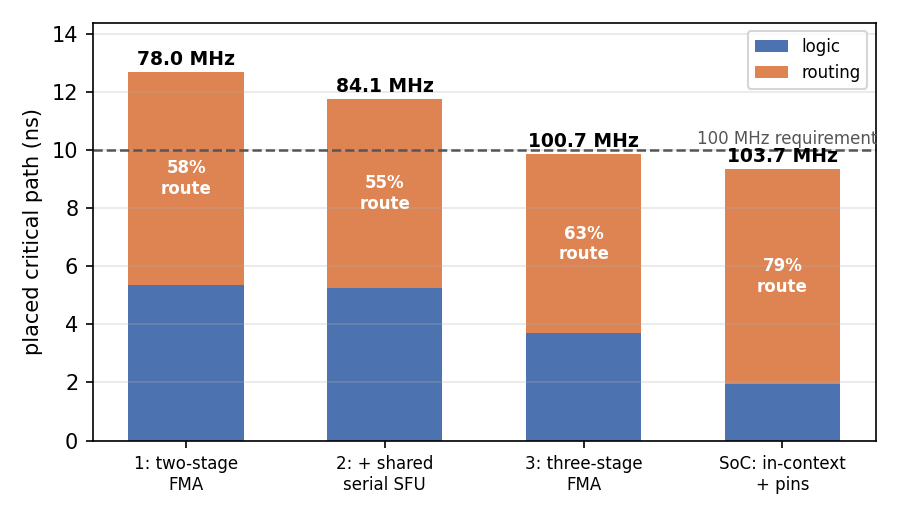
\includegraphics[width=\textwidth]{fp_closure.png}
      \end{center}
    \end{column}
  \end{columns}
\end{frame}

% ---- pdot8 -----------------------------------------------------------------
\begin{frame}{AI Extension --- the \texttt{pdot8} Custom Instruction}
  \begin{columns}[T]
    \begin{column}{0.54\textwidth}
      \begin{block}{What it computes}
        \small
        \[ rd \;=\; \sum_{i=0}^{3} \text{ext}(rs1.\text{byte}[i]) \times \text{ext}(rs2.\text{byte}[i]) \]
        Four packed INT8 MACs in one instruction. R-type, custom-0 opcode \texttt{0x0B}, \texttt{funct7}=0.
      \end{block}
      \begin{block}{Three signedness variants (\texttt{funct3})}
        \small
        \begin{tabular}{@{}lll@{}}
          \texttt{pdot8}   & S$\times$S & weights $\times$ weights \\
          \texttt{pdot8u}  & U$\times$U & activations $\times$ activations \\
          \texttt{pdot8su} & S$\times$U & \hl{weights $\times$ activations (inference)} \\
        \end{tabular}
      \end{block}
    \end{column}
    \begin{column}{0.46\textwidth}
      \begin{itemize}
        \item Emitted via \texttt{.insn} --- \hl{no compiler patch}, inert to existing kernels.
        \item Executes on the \navy{\texttt{W\_DOT}} DSP-pipelined background engine (4 DSPs/lane,
          $8\times4=32$ DSPs) --- \hl{off the critical path}.
        \item Non-accumulating (2-read-port VRF); the kernel accumulates with a separate \texttt{add}.
        \item The \hl{only} custom opcode in the whole project --- everything else is standard
          RISC-V.
      \end{itemize}
    \end{column}
  \end{columns}
\end{frame}

% ---- Quantized operators ---------------------------------------------------
\begin{frame}{Quantized Operator Library}
  \begin{columns}[T]
    \begin{column}{0.5\textwidth}
      \begin{itemize}
        \item \navy{\texttt{qgemm}} --- INT8 GEMM tile ($M{=}N{=}8$, $K{=}16$): one warp/row, one
          lane/col; the reduction runs 4-at-a-time on \texttt{pdot8}.
        \item \navy{\texttt{qgemv}} --- INT8 GEMV, one lane per output; parameterized $K,N$ so the
          \hl{same kernel} runs both MLP layers.
        \item \navy{\texttt{requant\_relu}} --- INT32$\rightarrow$INT8 rescale + ReLU, reusing the FPU
          (branchless \texttt{fmadd}+clamp), so \hl{no new hardware}.
      \end{itemize}
      \vspace{0.2em}
      {\footnotesize Layouts are chosen so both operand streams \hl{coalesce} and each stage's
      output is already the next stage's input format.}
    \end{column}
    \begin{column}{0.5\textwidth}
      \begin{block}{\texttt{qgemm} measured ($8{\times}8$, $K{=}16$)}
        \small
        \begin{tabular}{@{}lr@{}}
          \toprule
          Metric & Value \\
          \midrule
          MACs                 & 1024 \\
          Cycles               & 538 \\
          Throughput           & 1.90 MAC/cycle \\
          Global-mem txns      & 72 \\
          Naïve (uncoalesced)  & 576 \\
          \hl{Traffic reduction} & \hl{$8\times$} \\
          Correctness          & 64/64 bit-exact \\
          \bottomrule
        \end{tabular}
      \end{block}
      {\footnotesize Coalescing matches the analytic model exactly.}
    \end{column}
  \end{columns}
\end{frame}

% ---- MNIST pipeline --------------------------------------------------------
\begin{frame}{End-to-End MNIST Inference}
  A pre-trained INT8 MLP (\hl{$784 \to 128 \to 10$}) classifies MNIST digits using only the
  operators above:
  \vspace{0.4em}
  \begin{center}
  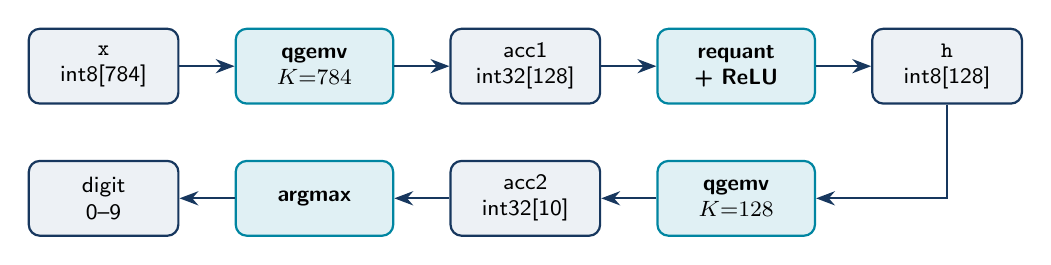
\begin{tikzpicture}[
      node distance=0.55cm and 0.7cm,
      box/.style={draw=simtixblue,fill=simtixlight,rounded corners,thick,
        minimum height=0.95cm,minimum width=1.9cm,align=center,font=\footnotesize},
      op/.style={draw=simtixaccent,fill=simtixaccent!12,rounded corners,thick,
        minimum height=0.95cm,minimum width=2.0cm,align=center,font=\footnotesize\bfseries},
      a/.style={-{Stealth[length=2.4mm]},thick,simtixblue}]
    \node[box] (x) {\texttt{x}\\int8[784]};
    \node[op,right=of x] (g1) {qgemv\\$K{=}784$};
    \node[box,right=of g1] (a1) {acc1\\int32[128]};
    \node[op,right=of a1] (rq) {requant\\+ ReLU};
    \node[box,right=of rq] (h) {\texttt{h}\\int8[128]};
    \node[op,below=0.7cm of rq] (g2) {qgemv\\$K{=}128$};
    \node[box,left=of g2] (a2) {acc2\\int32[10]};
    \node[op,left=of a2] (am) {argmax};
    \node[box,left=of am] (p) {digit\\0--9};
    \draw[a] (x)--(g1); \draw[a] (g1)--(a1); \draw[a] (a1)--(rq); \draw[a] (rq)--(h);
    \draw[a] (h.south) |- (g2.east);
    \draw[a] (g2)--(a2); \draw[a] (a2)--(am); \draw[a] (am)--(p);
  \end{tikzpicture}
  \end{center}
  \vspace{0.3em}
  \begin{columns}[T]
    \begin{column}{0.5\textwidth}
      \begin{block}{Accuracy (numpy-trained, quantized)}
        \small
        \begin{tabular}{@{}lr@{}}
          \toprule
          FP32 test accuracy  & 96.82\% \\
          INT8 test accuracy  & 96.53\% \\
          Quantization drop   & \hl{0.29\%} \\
          \bottomrule
        \end{tabular}
      \end{block}
    \end{column}
    \begin{column}{0.5\textwidth}
      \begin{block}{Hardware correctness}
        \small
        \begin{tabular}{@{}lr@{}}
          \toprule
          vs.\ integer golden & \hl{64 / 64 bit-exact} \\
          on 64-image subset  & 98.4\% (63/64) \\
          \bottomrule
        \end{tabular}
      \end{block}
    \end{column}
  \end{columns}
\end{frame}

% ---- On-chip MNIST demo ----------------------------------------------------
\begin{frame}{On-Chip Demo --- Host CPU Drives the Full Chip}
  \begin{columns}[T]
    \begin{column}{0.56\textwidth}
      \small
      The whole inference runs on the integrated \texttt{chip\_top}, exactly as a deployed chip would:
      \begin{itemize}
        \item Weights live in a \hl{256\,KB block-RAM store}; the host CPU \navy{streams} each weight
          tile into the 16\,KB LUTRAM working memory.
        \item CPU launches \texttt{qgemv}/\texttt{requant\_relu} per tile via MMIO, runs argmax,
          self-checks each digit against the on-chip golden.
        \item \hl{The accelerator core is untouched} --- BRAM's 1-cycle latency is hidden by a single
          CPU stall.
        \item \navy{Result: 64/64 bit-exact} on real hardware.
      \end{itemize}
    \end{column}
    \begin{column}{0.44\textwidth}
      \begin{center}
        \includegraphics[width=0.92\textwidth]{mnist_montage.png}\\[0.2em]
        {\footnotesize The 64 test images, classified on-chip.}
      \end{center}
    \end{column}
  \end{columns}
\end{frame}

% ---- FPGA results I --------------------------------------------------------
\begin{frame}{FPGA Implementation Results --- PPA (xczu7ev / ZCU104)}
  Three representative builds of the complete chip, all on the ZCU104's Zynq UltraScale+:
  \vspace{0.3em}
  \begin{center}\small
  \begin{tabular}{@{}lrrrr@{}}
    \toprule
    Build & LUT & FF & DSP & BRAM \\
    \midrule
    Integer baseline chip            & 34.3k & 6.2k  & 24 & 0 \\
    FP-enabled chip (deployable, routed) & 71.6k & --   & 40 & 0 \\
    \textbf{AI MNIST chip (INT8 + BRAM)} & \textbf{83.5k} & \textbf{18.9k} & \textbf{72} & \textbf{64} \\
    \bottomrule
  \end{tabular}
  \end{center}
  \vspace{0.4em}
  \begin{columns}[T]
    \begin{column}{0.5\textwidth}
      \begin{block}{Timing --- all meet 100\,MHz}
        \small
        \begin{tabular}{@{}lr@{}}
          Integer chip     & 100\,MHz (+0.25\,ns) \\
          FP chip (routed)  & \hl{103.7\,MHz}, 0 DRC \\
          AI MNIST chip     & 100\,MHz (+1.71\,ns) \\
        \end{tabular}
      \end{block}
    \end{column}
    \begin{column}{0.5\textwidth}
      \begin{block}{Power (vectorless)}
        \small
        \begin{tabular}{@{}lr@{}}
          Integer chip  & 0.96\,W \\
          FP chip       & 1.20\,W \\
          AI MNIST chip & 1.36\,W \\
        \end{tabular}
      \end{block}
    \end{column}
  \end{columns}
\end{frame}

% ---- FPGA results II: MNIST BRAM highlight --------------------------------
\begin{frame}{FPGA Results --- The AI MNIST Chip (Newest)}
  \begin{columns}[T]
    \begin{column}{0.52\textwidth}
      \begin{block}{Utilization (OOC synthesis)}
        \small
        \begin{tabular}{@{}lrr@{}}
          \toprule
          Resource & Used & Util.\ \% \\
          \midrule
          CLB LUTs           & 83{,}475 & 36.2 \\
          \; LUT as logic    & 69{,}247 & 30.1 \\
          \; LUT as memory   & 14{,}228 & 14.0 \\
          CLB registers      & 18{,}939 & 4.1 \\
          \textbf{Block RAM (RAMB36)} & \textbf{64} & \textbf{20.5} \\
          DSP                & 72 & 4.2 \\
          \bottomrule
        \end{tabular}
      \end{block}
    \end{column}
    \begin{column}{0.48\textwidth}
      \begin{itemize}
        \item \hl{First non-zero BRAM} in the project: the 256\,KB weight store (2\,Mbit) maps to
          \navy{64 RAMB36} tiles, initialised bit-exact from the trained weights.
        \item \navy{72 DSP} = FP fabric's 40 + \texttt{pdot8}'s 32 INT8 MAC DSPs.
        \item \navy{100\,MHz met} with +1.71\,ns slack; power \textbf{1.36\,W}.
        \item Verified by a \hl{post-synthesis gate-level simulation} of the synthesized netlist.
      \end{itemize}
    \end{column}
  \end{columns}
\end{frame}

% ---- Energy efficiency -----------------------------------------------------
\begin{frame}{Energy Efficiency --- Honest Positioning}
  \begin{columns}[T]
    \begin{column}{0.55\textwidth}
      \begin{block}{INT8 efficiency (measured, @100\,MHz)}
        \small
        \begin{tabular}{@{}lrr@{}}
          \toprule
          & Throughput & Efficiency \\
          \midrule
          Measured (\texttt{qgemm}) & 0.38 GOP/s & 0.39 GOP/s/W \\
          Datapath ceiling          & 6.4 GOP/s  & 6.6 GOP/s/W \\
          \bottomrule
        \end{tabular}
      \end{block}
      \vspace{0.2em}
      {\footnotesize For an 8-lane academic core these land honestly in the \hl{GOPS} range
      (milli-TOPS) --- the point is a \emph{correct, coalesced, measured} baseline, not peak density.}
    \end{column}
    \begin{column}{0.45\textwidth}
      \begin{block}{The gap $\Rightarrow$ future work}
        \small The measured-vs-ceiling gap comes from the single-slot dot engine and per-warp
        dependency chains. The lever for real density is a \hl{tensor / systolic engine}
        (Tier-3), not more SIMT tuning --- \texttt{qgemm} defines the baseline it will be measured
        against.
      \end{block}
    \end{column}
  \end{columns}
\end{frame}

% ---- Verification ----------------------------------------------------------
\begin{frame}{Verification \& Methodology}
  \begin{columns}[T]
    \begin{column}{0.5\textwidth}
      \begin{block}{Functional verification}
        \small
        \begin{itemize}
          \item 14-testbench regression, all green.
          \item \hl{$>$116{,}000 bit-exact} FP self-checks against a DPI reference (FP32 + FP16,
            all ops incl.\ FMA, div/sqrt).
          \item Golden-model checks for every quantized kernel and the full MNIST pipeline.
        \end{itemize}
      \end{block}
    \end{column}
    \begin{column}{0.5\textwidth}
      \begin{block}{Silicon-accurate verification}
        \small
        \begin{itemize}
          \item \navy{Post-synthesis} gate-level simulation of the synthesized netlist.
          \item \navy{Post-implementation} functional sim of the \hl{routed} netlist --- proves
            the real placed-and-routed hardware computes correctly.
          \item Clean-DRC bitstream with real ZCU104 pin constraints.
        \end{itemize}
      \end{block}
    \end{column}
  \end{columns}
  \vspace{0.3em}
  {\footnotesize Tooling: Verilator (fast RTL regression) + Xilinx Vivado 2025.1 (synthesis,
  implementation, gate-level xsim); RISC-V GNU toolchain for kernels.}
\end{frame}

% ---- DSE -------------------------------------------------------------------
\begin{frame}{Design-Space Exploration --- Key Findings}
  \begin{itemize}
    \item \navy{Lane count is not the Fmax lever.} Halving the fabric (4 vs 8 lanes) did \hl{not}
      improve placed Fmax --- the critical path is a \emph{single} lane's FMA cone, independent of
      lane count. 8 lanes Pareto-dominates 4 (same Fmax, $2\times$ throughput).
    \item \navy{The FP fabric is interconnect-bound.} At $\sim$31\% device utilization the binding
      constraint is \hl{routing / congestion}, not logic depth --- confirmed by the shared-SFU
      de-congestion win (+6\,MHz from identical logic).
    \item \navy{FMA microarchitecture is the real lever.} A 3-stage FMA (attacking logic depth of the
      binding cone) is what finally closed 100\,MHz; the path then moved off the FMA entirely onto
      the register-file read mux --- the same limiter as the integer design.
  \end{itemize}
  \vspace{0.2em}
  {\footnotesize A full diagnose $\rightarrow$ confirm $\rightarrow$ localize $\rightarrow$ fix arc,
  with every step measured on placed-and-routed hardware.}
\end{frame}

% ---- Contributions ---------------------------------------------------------
\begin{frame}{Key Contributions}
  \begin{enumerate}
    \item A complete, open, \hl{programmable RISC-V SIMT accelerator} (8 lanes $\times$ 4 warps)
      with true reconvergence, coalescing, and park-and-resume latency hiding.
    \item A \hl{FP32 + FP16} subsystem (NaN-boxed shared file, pipelined FMA, shared div/sqrt) that
      closes 100\,MHz --- with an honest, measured \navy{timing-closure study} showing the design is
      interconnect-bound.
    \item An \hl{AI-inference extension}: a single custom INT8 dot-product instruction, a quantized
      operator library (GEMM/GEMV/requant), and an \navy{end-to-end MNIST} demo that is
      \textbf{64/64 bit-exact on hardware}.
    \item A \hl{full RTL-to-bitstream flow} on the ZCU104 with silicon-accurate verification and a
      complete PPA characterization across integer, FP, and INT8+BRAM builds.
  \end{enumerate}
\end{frame}

% ---- Status ----------------------------------------------------------------
\begin{frame}{Current Status --- Results Summary}
  \begin{center}\small
  \begin{tabular}{@{}lll@{}}
    \toprule
    Aspect & Result & Status \\
    \midrule
    SIMT core (int)        & 8$\times$4, coalescing, divergence   & \color{simtixgreen}\textbf{done} \\
    FP32 / FP16 subsystem  & all ops, pipelined FMA, div/sqrt     & \color{simtixgreen}\textbf{done} \\
    Timing closure         & 100.7\,MHz placed / 103.7\,MHz SoC   & \color{simtixgreen}\textbf{done} \\
    Custom \texttt{pdot8}  & INT8 4-way dot, 3 variants, DSP eng. & \color{simtixgreen}\textbf{done} \\
    Quantized operators    & \texttt{qgemm}/\texttt{qgemv}/requant, coalesced & \color{simtixgreen}\textbf{done} \\
    End-to-end MNIST       & 96.53\% INT8, 64/64 bit-exact on HW  & \color{simtixgreen}\textbf{done} \\
    AI chip PPA (+BRAM)    & 83.5k LUT / 64 BRAM / 72 DSP, 100\,MHz & \color{simtixgreen}\textbf{done} \\
    Verification           & 14-tb + 116k FP checks + gate-level  & \color{simtixgreen}\textbf{done} \\
    \bottomrule
  \end{tabular}
  \end{center}
  \vspace{0.4em}
  {\footnotesize All milestones RTL-complete, FPGA-implemented, and verified; the M.Tech.\ thesis
  documents each build with its measured tables.}
\end{frame}

% ---- Future work -----------------------------------------------------------
\begin{frame}{Future Work}
  \begin{columns}[T]
    \begin{column}{0.5\textwidth}
      \begin{block}{Near term}
        \small
        \begin{itemize}
          \item Chip-level place-and-route of the MNIST build for a placed Fmax + bitstream.
          \item ZCU104 \hl{board bring-up} of the on-chip demo.
          \item Shrink the register-file read mux (now the shared FP/int critical path).
        \end{itemize}
      \end{block}
    \end{column}
    \begin{column}{0.5\textwidth}
      \begin{block}{Longer term}
        \small
        \begin{itemize}
          \item \hl{Tier-3 tensor / systolic engine} --- output-stationary MAC array for real
            TOPS-class density (weight-sharing DSP packing).
          \item Dedicated integer requantize engine (FPU-less INT8 path).
          \item \hl{Open-source sky130 GDS} (RTL-to-GDS) for an ASIC data point.
        \end{itemize}
      \end{block}
    \end{column}
  \end{columns}
\end{frame}

% ---- Thank you -------------------------------------------------------------
{
\setbeamertemplate{footline}{}
\begin{frame}[plain]
  \vspace{1.4cm}
  \begin{center}
    {\color{simtixaccent}\rule{0.8\textwidth}{1.0pt}}\\[0.8em]
    {\Huge\bfseries\color{simtixblue} Thank you}\\[0.7em]
    {\large\color{simtixblue} SIMTiX --- a RISC-V SIMT accelerator that runs a real
     quantized network end-to-end on measured hardware}\\[0.7em]
    {\color{simtixaccent}\rule{0.8\textwidth}{1.0pt}}\\[1.2em]
    {\normalsize Questions \& discussion}\\[0.6em]
    {\footnotesize Krishna Gorai \quad$\cdot$\quad M.Tech., IIT Mandi}
  \end{center}
\end{frame}
}

\end{document}
